%-----------------------------------------------------------------------
% Copyright (c) 2011-2017  Remko Scharroo
% See LICENSE.TXT file for copying and redistribution conditions.
%
% This program is free software: you can redistribute it and/or modify
% it under the terms of the GNU Lesser General Public License as
% published by the Free Software Foundation, either version 3 of the
% License, or (at your option) any later version.
%
% This program is distributed in the hope that it will be useful,
% but WITHOUT ANY WARRANTY; without even the implied warranty of
% MERCHANTABILITY or FITNESS FOR A PARTICULAR PURPOSE.  See the
% GNU Lesser General Public License for more details.
%-----------------------------------------------------------------------

\documentclass[a4paper,11pt,openany,natbib,nomargin]{thesis}
\usepackage{palatino}
\usepackage{newpxmath}
\usepackage{verbatim}
\usepackage{graphicx}
\usepackage{rads}
\usepackage{makeidx}
\usepackage{url}\urlstyle{sf}
\usepackage{rotating}
\usepackage{placeins}
\bibliographystyle{agu08}
\input{rads_config}

\DeclareUrlCommand\cmd{\urlstyle{tt}}
\renewcommand\deg{\ensuremath{^\circ}}
\newcommand\prog[1]{\url{#1}\index{programs!#1@\protect\url{#1}}}
\DeclareUrlCommand\code{\urlstyle{tt}}
\newcommand\Code[1]{\textbf{\code{#1}}}
\newcommand\CODE[1]{\Code{\emph{#1}}}
\newcommand\file[1]{\url{#1}\index{files!#1@\protect\url{#1}}}
\newcommand\cc[1]{\multicolumn{1}{c}{\em #1}}
\newcommand\var[1]{\url{#1}\index{variables!#1@\protect\url{#1}}}
\newcommand\alias[1]{\emph{alias of} \var{#1}}
\setcounter{topnumber}{3}
\renewcommand{\topfraction}{.9}
\setcounter{bottomnumber}{2}
\renewcommand{\bottomfraction}{.7}
\setcounter{totalnumber}{4}
\renewcommand{\textfraction}{.1}
\renewcommand{\floatpagefraction}{.8}

\newenvironment{vartable}{
\begin{table}[ht]
\small
\begin{tabular}{lrllllr}
\hline
Variable & field & name & units & sat & range & note \\
\hline
}{
\hline
\end{tabular}
\end{table}
}

\verbatimfont{\small}
\newenvironment{notes}[1][Notes:]{\FloatBarrier\paragraph{#1}\begin{enumerate}}{\end{enumerate}}

%%%%%%%%%%%%%%%%%%%%%%%%%%%%%%%%%%%%%%%%%%%%%%%%%%%%%%%%%%%%%%%%

\makeindex

\title{RADS Data Manual}
\author{Remko Scharroo}
\date{Version \vernum\\\today}

\begin{document}

\maketitle
\tableofcontents

%%%%%%%%%%%%%%%%%%%%%%%%%%%%%%%%%%%%%%%%%%%%%%%%%%%%%%%%%%%%%%%%

\chapter{Introduction}
\label{ch:intro}
This manual is intended to explain the details about the many variables available in the RADS data base. Many of the variables come in different "flavours", like one could choose to use the wet tropospheric correction based on radiometer measurements (\var{wet_tropo_rad}) or one of the atmospheric models (e.g., \var{wet_tropo_ecmwf}). RADS also provides the option to use more generic variable names (like \var{wet_tropo}) that will pick the best available correction depending on the satellite mission (or period).

The variables are organised various chapters. Consult the table of contents to find the variables you are looking for, or go to the index at the end of the manual, where all variables are listed.

\begin{table}
\begin{tabular}{lccll}
\hline
Altimeter & Abbr. & Nr & Alternatives & References \\
\hline
GEOS 3      & g3 &  1 & ge3 geos-3 geos3                    & (not included in RADS) \\
Seasat      & ss &  2 & sea seasat-a                        & (not included in RADS) \\
Geosat      & gs &  3 & geo geosat                          & \\
ERS-1       & e1 &  4 & er1 ers-1 ers1                      & \citep{francis1990a,francis1991a} \\
TOPEX       & tx &  5 & top topex                           & \citep{fu1994} \\
Poseidon    & pn &  6 & pos poseidon                        & \\
ERS-2       & e2 &  7 & er2 ers-2 ers2                      & \citep{francis1995a} \\
GFO         & g1 &  8 & gfo gfo-1 gfo1                      & \\
Jason-1     & j1 &  9 & ja1 jason-1 jason1                  & \citep{menard2003} \\
Envisat     & n1 & 10 & en1 envisat                         & \\
Jason-2     & j2 & 11 & ja2 jason-2 jason2                  & \citep{lambin2010} \\
CryoSat-2   & c2 & 12 & cs2 cryosat-2 cryosat2              & \citep{wingham2006} \\
SARAL       & sa & 13 & sa srl saral altika                 & \\
Jason-3     & j3 & 14 & ja3 jason-3 jason3                  & \\
HY-2A       & 2a & 15 & h2a hy-2a hy2a                      & (not included in RADS) \\
Sentinel-3A & 3a & 16 & s3a sentinel-3a sentinel3a sntnl-3a & \\
Sentinel-3B & 3b & 17 & s3b sentinel-3b sentinel3b sntnl-3b & (limited access in RADS) \\
\hline
\end{tabular}
\caption{Abbreviation and numbers used for the various altimeter missions.}
\label{tab:rads4_sats}
\end{table}


For each variable, a list of different flavours is presented. For an example, turn to Section~\ref{var:wet_tropo}. This Section describes the various wet tropospheric corrections. The table in that Section lists in the first column the various variable names, followed by the field number as was used in RADS 3 (and can still be used in RADS 4), a short description, and the units of this variable. The next column lists for which altimeter missions this variable is available (see Table~\ref{tab:rads4_sats}), where "all" stands of all missions, and "other" stands for all missions not mentioned above it. The second to last column is the default range used for editing (NaN is returned when the value exceeds this range). When this column is empty, no range limits are set. Finally, the rightmost column relates to a list of notes provided in that Section.

Near the bottom of each variable table a number of "aliases" are provided. These are short-cuts to one (or more) of the flavours of variables. For example, the tables in Section~\ref{var:wet_tropo} shows that for most altimeter missions the alias \var{wet_tropo} means that radiometer wet tropospheric correction is used (\var{wet_tropo}), but, when not available, for example during extended outage, the ECMWF model wet tropospheric correction (\var{wet_tropo_ecmwf}) is used instead. These "aliases" make it easier to get the preferred flavour of the variable which may differ from mission to mission (for example, some do not have a radiometer). This largely simplifies the construction of sea level anomalies, as described in Section~\ref{var:sla}.

\chapter{Time and location}
\label{ch:time and location}

\section{Time}
\label{var:time}
Time in the RADS data sets is stored as 8-byte floats in UTC seconds since a given epoch (normally 1 January 1985 or 1 January 2000). RADS will automatically convert these values into a few common time scales, depending on which time variable is selected.
However, irrespective of the time scale, the clock references to UTC, rather than an atomic clock, meaning that leap seconds may result in a duplication of measurement times. No provision has been made to avoid confusion between measurements made before and after a leap second.

The time corresponds to the moment of reflection of the radar pulse on the sea surface and is corrected for time tag biases.

\begin{vartable}
\var{time_1985} & 101 & time since 1985-01-01 00:00:00 & s & all & & \\
\var{time_2000} & 106 & time since 2000-01-01 00:00:00 & s & all & & \\
\var{time_rel_eq} & 102 & time relative to equator crossing & s & all & & \ref{item:time_rel_eq} \\
\var{time_local_solar} & 103 & local solar time & s & all & & \ref{item:time_local_solar} \\
\var{time_mjd} & 105 & time since 1858-11-17 00:00:00 & days & all & & \ref{item:time_mjd} \\
\var{time_ymdhms} & 104 & time formatted as ymdhms &  & all & & \ref{item:time_ymdhms} \\
\hline
\var{time} & 1 & \alias{time_1985} & & all & & \ref{item:time} \\
\end{vartable}

\begin{notes}
\item Time is negative prior to equator crossing, positive thereafter.\label{item:time_rel_eq}
\item The local solar time is expressed as seconds since the start of the day.\label{item:time_local_solar}
\item Time in Modified Julian Days.\label{item:time_mjd}
\item The variable \var{time_ymdhms} will produce a floating value of the type 20110908135001.536 for 8 Sep 2011 13:50:01.536 UTC.\label{item:time_ymdhms}
\item No time limit is set by default. Can be controlled by the \cmd{--t} or \cmd{--ymd} flags on the command line.\label{item:time}
\item A time tag bias (surplus) of 1.8 ms was removed from the time tags of ERS-1 as they occurred on the ESA OPR (Ocean Product) data product. Likewise, all time tags of ERS-2 were decreased by 1.3 ms. The orbital altitude and location has been adjusted accordingly.
\end{notes}

\section{Latitude and longitude}
The position of the centre of the footprint of the measurement is given by its geographical longitude and latitude relative the TOPEX reference ellipsoid. Longitude is in degrees relative to the Greenwich meridian, positive measuring east. Latitude is in degrees relative to the equator, positive measuring north.

\begin{vartable}
\var{lat} & 2, 201 & latitude & degrees north & all & -90 90 & \\
\var{lon} & 3, 301 & longitude & degrees east & all & -180 180 & 1 \\
\end{vartable}

\begin{notes}[Note:]
\item RADS will automatically adjust the values to be within the range specified. So, by default, longitudes are kept within the -180 to +180 range.
\end{notes}

\section{Orbital altitude}\label{var:alt}
The orbital altitude is the height of the centre-of-mass of the satellite above the TOPEX reference ellipsoid (semi-major axis = 6378136.3 m, inverse flattening = 298.257) as computed by satellite orbit determination. Numerous solutions exist, based on varying combinations of tracking data or gravity field solutions, or computed at shorter or longer latency. Some "legacy solutions" (those that were provided on the original data products) are included for reference even when they have been long replaced by more accurate solutions.

The altitude is that of the centre-of-mass of the spacecraft, so corrections from the tracking devices (DORIS, GPS, PRARE, SLR) to the centre-of-mass, as well as motion of the centre-of-mass within the spacecraft are accounted for, and should also be accounted for when later subtracting the altimeter range referenced to the same point.

If the time tags on the original GDR data include a bias, the orbit has either been (re)interpolated at the \emph{corrected} time tag, or a correction proportional to the orbital altitude rate has been applied.

\begin{vartable}
\var{alt_jgm3}     & 401 & JGM-3 altitude   & m & gs pn tx && \ref{item:alt_jgm3} \\
\var{alt_dgme04}   & 402 & DGM-E04 altitude & m & e1 e2 && \ref{item:alt_dgme04} \\
\var{alt_cnes}     & 404 & CNES altitude    & m & c2 n1 pn tx && \ref{item:alt_cnes} \\
\var{alt_pgs7777}  & 410 & PGS7777 altitude  & m & g1 && \ref{item:alt_pgs7777} \\
\var{alt_ggm02c_itrf2000}& 411 & GGM02c(ITRF2000) altitude  & m & gs pn tx && \ref{item:alt_ggm02c} \\
\var{alt_ggm02c_itrf2005}& 413 & GGM02c(ITRF2005) altitude  & m & pn tx && \ref{item:alt_ggm02c} \\
\var{alt_eiggl04s} & 414 & EIGEN-GL04c altitude & m & j1 && \ref{item:alt_eiggl04s} \\
\var{alt_gdrcp}    & 415 & GDR-C' altitude & m & g1 gs j1 j2 n1 pn tx && \ref{item:alt_gdrcp} \\
\var{alt_gps}      & 416 & GPS altitude & m & j1 j2 && \ref{item:alt_gps} \\
\var{alt_eig6c}    & 417 & EIGEN-6C altitude & m & c2 n1 && \ref{item:alt_eig6} \\
\var{alt_eig6s2}   & 417 & EIGEN-6S2 altitude & m & j1 j2 && \ref{item:alt_eig6} \\
\var{alt_gdrd}     & 418 & CNES GDR-D altitude & m & c2 j1 j2 n1 sa && \ref{item:alt_gdrd} \\
\var{alt_std1204}  & 419 & GSFC/Std1204 altitude & m & j1 j2 pn tx && \ref{item:alt_std1204} \\
\var{alt_reaper}   & 420 & REAPER/COMBI altitude & m & e1 e2 && \ref{item:alt_reaper} \\
\var{alt_reaper_deos} & 421 & REAPER/DEOS altitude & m & e1 e2 && \ref{item:alt_reaper} \\
\var{alt_reaper_gfz}  & 422 & REAPER/GFZ altitude & m & e1 e2 && \ref{item:alt_reaper} \\
\var{alt_reaper_esoc} & 423 & REAPER/ESOC altitude & m & e1 e2 && \ref{item:alt_reaper} \\
\var{alt_std1404}  & 424 & GSFC/Std1404 altitude & m & j2 && \ref{item:alt_std1404} \\
\var{alt_gdre}     & 425 & CNES GDR-E altitude & m & c2 j2 j3 sa && \ref{item:alt_gdre} \\
\var{alt_slcci}    & 426 & GFZ/SLCCI altitude & m & e1 e2 j1 j2 n1 pn tx && \ref{item:alt_slcci} \\
\hline
\var{alt} & 4 & \alias{alt_gdre} \var{alt_cnes} & & c2 && \ref{item:alt}\\
\var{alt} & 4 & \alias{alt_reaper} \var{alt_gfz} & & e1 e2 && \ref{item:alt} \\
\var{alt} & 4 & \alias{alt_pgs7777} & & g1 && \ref{item:alt} \\
\var{alt} & 4 & \alias{alt_gdrcp} & & gs && \ref{item:alt} \\
\var{alt} & 4 & \alias{alt_gdre} & & j1 && \ref{item:alt} \\
\var{alt} & 4 & \alias{alt_gdre} \var{alt_gdrd} & & j2 && \ref{item:alt} \\
\var{alt} & 4 & \alias{alt_gdre} & & j3 sa && \ref{item:alt} \\
\var{alt} & 4 & \alias{alt_gdrd} \var{alt_gdrcp} & & n1 && \ref{item:alt} \\
\var{alt} & 4 & \alias{alt_gdrcp} \var{alt_jgm3} & & pn tx && \ref{item:alt} \\
\end{vartable}

\begin{notes}
\item JGM-3 \citep{tapley1996} was the original gravity field solutions used by NASA for the orbit determination of Geosat and TOPEX/Poseidon that featured on the GDR products. Though the gravity field was tailored to the TOPEX orbit, it was generally regarded the best at the time and was hence also used more widely than just for TOPEX/Poseidon. The radial orbit accuracy of about 3 cm for TOPEX/Poseidon and 8 cm for Geosat has since been superseded by more up-to-date orbit solutions.\label{item:alt_jgm3}
\item DGM-E04 was a gravity field model developed at the Delft University of Technology tailored to the ERS-1 and ERS-2 orbits and derived from the JGM-3 model. The model significantly improved the radial orbit accuracy to about 3.5 cm, better than any general purpose models available at the time \citep{scharroo1998a}.\label{item:alt_dgme04}
\item CNES produces the operational and precise orbits for a number of satellites. Unfortunately, in RADS the CNES orbits are based on mix of gravity field solutions. The CNES orbits for the TOPEX/Poseidon mission feature on the GDRs and are based on the JGM-3 gravity field model \citep{tapley1996}. The CNES orbits for CryoSat and Envisat are obtained from their respective GDR products and are based on the EIGEN-GL04c gravity field model \citep{ablain2008}.\label{item:alt_cnes}
\item PGS7777 is a NASA preliminary gravity field solution tailored to the Geosat and GFO satellite orbits. The NASA PGS7777 orbit solution for GFO \citep{lemoine2006a} is based on SLR data only as the GPS tracking system on GFO failed.\label{item:alt_pgs7777}
\item Orbit solutions created at NASA using the GGM02c gravity field and station coordinates in the ITRF2000 or ITRF2005 reference frame.\label{item:alt_ggm02c}
\item Orbits produced with the EIGEN-GL04c or EIGEN-GL04s gravity fields.\label{item:alt_eiggl04s}
\item Orbits produced under strict Jason GDR-C' standards.\label{item:alt_gdrcp}
\item Reduced-dynamic (fast-delivery) orbits based on GPS tracking data only.\label{item:alt_gps}
\item Orbits provided by ESOC using the EIGEN-6C or EIGEN-6S2 gravity field. The orbits are available for parts of the various altimeter missions only: CryoSat-2 cycles 4-58, Envisat all cycles, Jason-1 cycles 1-260, Jason-2 cycles 1-220.\label{item:alt_eig6}
\item Orbits produced by CNES under strict Jason GDR-D standards \citep{ids2011}. These orbits are kept on Jason-2 data (until April 2015) and SARAL data (until June 2015) for comparison, although the GDR-E orbits are now default. Jason-1 data does not have GDR-E orbits yet.\label{item:alt_gdrd}
\item Orbits provided by GSFC using their standards "Std1204". They are "GDR-D compatible" and use the goce2s\_fit2 gravity field \citep{lemoine2013}.\label{item:alt_std1204}
\item Orbits produced by the REAPER project. A combined solution and individual solutions created by DEOS (TU Delft), GFZ and ESOC are available \citep{rudenko2011}.\label{item:alt_reaper}
\item Orbits provided by GSFC using their standards "Std1404". They are "GDR-E compatible".\label{item:alt_std1404}
\item Orbits produced by CNES under strict Jason GDR-E standards (baseline for the production of orbits since April 2015) \citep{ids2015}.\label{item:alt_gdre}
\item Orbits produced by GFZ in the framework of the ESA Sea Level CCI project. RADS initially included version VER06 of these orbits (based on the EIGEN-6S2A gravity field model) \citep{rudenko2014} for ERS-1, ERS-2, Envisat and TOPEX/Poseidon. Any data produced since 18 May 2016 (which includes Jason-1 and Jason-2) incorporated version VER11 of these orbits and are based on the EIGEN-6S4 gravity field model \citep{rudenko2015,rudenko2016}.\label{item:alt_slcci}
\item The variable \var{alt} refers to the preferred (best) orbit solution for each satellite. If two variable names are mentioned, RADS picks the first one by preference; it that is not available, the second variable is used.\label{item:alt}
\end{notes}

\section{Orbital altitude rate}
The rate of change of the orbital altitude is relevant for computing the Doppler correction and for correcting the altitude as a result of a time tag bias. Furthermore, the orbital altitude rate can be used to estimate time tag biases.

\begin{vartable}
\var{alt_rate} & 5, 501 & orbital altitude rate & m/s & all && \\
\end{vartable}

\chapter{Sea level variables}
\section{Sea level anomaly}
\label{var:sla}
The sea level anomaly (SLA) or sea surface height anomaly (SSHA) is the height for the sea surface relative to a long term mean. It can be constructed by subtracting from the satellite orbital altitude the altimeter range, propagation corrections, sea state bias, tides, and a mean sea surface model.

The sea level anomaly in RADS is always computed on-the-fly. This means that the RADS software will gather the required variables and their selected flavours from the netCDF data files, edit those data based on the user-selected criteria, and then constructs the sea level anomaly based on those. If any of the variables that make up the sea level anomaly is not available, marked invalid, or is out of range, then the sea level anomaly is also marked invalid (set to the NaN value). In addition, variables that do not strictly make up the sea level anomaly (like wave height or wind speed) can be used as edit criteria, e.g. rejecting data with high sea states.

The \file{rads.xml} configuration file spells out, in reverse polish notation (RPN), how the sea level anomaly (\var{sla}) is computed. The 'sea level equation' is written as:

\begin{verbatim}
<data>
    alt range SUB dry_tropo SUB wet_tropo SUB iono SUB
    dac SUB tide_solid SUB tide_ocean SUB tide_load SUB
    tide_pole SUB ssb SUB mss SUB ref_frame_offset SUB
</data>
\end{verbatim}

where \cmd{SUB} stands for 'subtract' and the others are names or aliases of the various variables that make up the sea level anomaly. If any of these variables is NaN, the result is NaN as well.
The use of aliases comes in handy here. We can, for example, switch out the orbit solution between one flavour
and another simply by directing the alias \var{alt} from say \var{alt_jgm3} to \var{alt_dgme04}. We do not have to change anything to the sea level equation.

The configuration file also spells out which variables are used as 'quality flag'. That is, if any of these variables is set to NaN, the sea level anomaly is also set to NaN, even though these variables are not added or subtracted as part of the 'sea level equation'. For example:
\begin{verbatim}
<quality_flag>
    swh sig0 range_rms range_numval flags
</quality_flag>
\end{verbatim}

While the sea level anomaly variable \var{sla} is computed on-the-fly by the RADS software, there is a second variable \var{ssha} that is already stored on the RADS products. Users can use this variable directly as well, but then give up the opportunity to edit the results themselves.

\begin{vartable}
\var{sla} & 0 & sea level anomaly & m & all & -5 5 & \ref{item:sla} \\
\var{ssha} & & sea level anomaly (precomputed) & m & all & & \ref{item:ssha} \\
\end{vartable}

\begin{notes}
\item The limits on the sea level anomaly can be changed in the configuration file, of by using the \cmd{--sla=MIN,MAX} option on the command line.\label{item:sla}
\item The variable \var{ssha} is read directly from the RADS products and already is screened by editing.\label{item:ssha}
\end{notes}

\section{Altimeter range}
\label{var:range}
The range between the satellite and the sea surface is based on the total travel time of the radar pulse divided by twice the speed of light. This range is then corrected for internal paths within the instrument (internal calibration), variations in the frequency of the ultra-stable oscillator (USO correction), and the distance between the antenna and the satellite centre of mass (centre-of-mass offset). The range is further corrected for the Doppler effect. As such the range measures the distance between the satellite centre of mass and the sea surface, except for path delays in the atmosphere and sea surface interactions.

To compute the height of the sea surface, we subtract the primary range (generally Ku-band) from the satellite orbital altitude and then further correct for path delays and other corrections.

Dual-frequency altimeters measure the range also on a secondary frequency (C- and S-band) which allows for the computation of the ionospheric path delay directly for altimeter observations rather than models.

\begin{vartable}
\var{range_ka} & 601 & altimeter range (Ka) & m & sa & & \\
\var{range_ku} & 601 & altimeter range (Ku) & m & other & & \\
\var{range_ku_mle3} & 601 & altimeter range (MLE3) & m & j2 j3 & & \ref{item:range_ku_mle3} \\
\var{range_c}  & 602 & altimeter range (C) & m & tx j1 j2 j3 & & \\
\var{range_s}  & 602 & altimeter range (S) & m & n1 & & \\
\hline
\var{range} & 6 & \alias{range_ka} & & sa & & \\
\var{range} & 6 & \alias{range_ku} & & other & & \\
\end{vartable}

\begin{notes}
\item A constant bias of -124 mm is added to the Geosat range. An additional internal calibration and USO correction comes from an external file [\emph{Brian Beckley}, priv.\ comm., 2002].
\item The range of the ERS-1 and ERS-2 altimeters has been corrected for SPTR bias jumps and USO drift based on offline tables \citep{martini2000}.
\item A constant bias of 409.2 mm is added to the ERS-1 range \citep{francis1993b,stum1998a}.
\item The ERS-2 USO correction appears to be low during the periods 1997-07-26 20:24:04 to 1998-01-07 03:58:09 and 1998-03-17 11:10:48 to 2000-01-08 06:04:13. During both periods 4.77 mm is added to the USO correction (and to range).
\item The USO correction for Envisat is based on external USO correction files (1-Hz data): \url{http://earth.esa.int/pcs/envisat/ra2/auxdata/}
\item Even though the Envisat Ku- and S-band ranges have biases of the order of 45 cm, this is not corrected for in the range, but in the reference frame offset (\var{ref_frame_offset}). A correction of 150 mm is added to the S-band range to account for a bias in the dual-frequency ionosphere correction \citep{scharroo2010a}. During the short operation of the Side B altimeter, an additional 9 mm was added to both Ku- and S-band ranges.
\item S-band range for Envisat is available only until the loss of the S-band signal.
\item TOPEX Ku- and C-band ranges are corrected for internal path delays and oscillator drifts based on external correction files (one value per cycle: \url{http://topex.wff.nasa.gov/}) \citep{hayne1994}. An additional -15.4 mm is added to the C-band range to account for a bias in the dual-frequency ionosphere correction \citep{scharroo2010a}.
\item A constant bias of -2.3 mm is added to the Jason-1 C-band range to account for a bias in the dual-frequency ionosphere correction \citep{scharroo2010a}.
\item A separate range based on an MLE3 retracker is available for Jason-2 and -3.\label{item:range_ku_mle3}
\end{notes}

\section{Altimeter range statistics}
The altimeter ranges are provided in RADS as (approximately) 1-second averages based on 10, 20, or 40 'elementary' measurements during that second. The altimeter range reported is, in fact, not the statistical mean, but is generally determined as follows:
\begin{itemize}
\item Interpolate the orbital altitude at the same time tags as the elementary measurements;
\item Subtract the orbital altitude from the range;
\item Fit a linear trend true `range minus orbit';
\item Remove the linear trend;
\item Compute the standard deviation of the residuals (using $n-2$ in the denominator) where $n$ is the number of elementary measurements during a 1-Hz period;
\item Evaluate the linear trend at the mid point and add the local orbital altitude back at this point to obtain the average range.
\end{itemize}
Hence, technically, \var{range_rms} is not the standard deviation of the altimeter range, but the standard deviation of the elementary `orbit minus range' values with a trend fitted and removed as well, and taking into account the extra degree of freedom. It should also not be confused with an error estimate for the range measurement.

\begin{vartable}
\var{range_rms_ka} & 2002 & std dev of Ka-band range & m & sa & 0.0 0.17 & \\
\var{range_rms_ku} & 2002 & std dev of Ku-band range & m & g1 gs & 0.0 0.25 & \\
                   &      &                          &   & j1 & 0.0 0.2 & \\
                   &      &                          &   & j2 j3 & 0.0 0.17 & \\
                   &      &                          &   & tx & 0.0 0.15 & \\
                   &      &                          &   & other & 0.0 0.4 & \\
\var{range_rms_c}  & 2004 & std dev of C-band range  & m & j1 j2 j3 & 0.0 0.4 & \\
\var{range_rms_s}  & 2004 & std dev of S-band range  & m & n1 & 0.0 0.4 & \ref{item:range_rms_s} \\
\hline
\var{range_rms}    &   20 & \alias{range_rms_ka} && sa && \\
\var{range_rms}    &   20 & \alias{range_rms_ku} && other && \\
\end{vartable}

\begin{notes}[Note:]
\item Standard deviation of S-band range for Envisat is available only until the loss of the S-band signal.\label{item:range_rms_s}
\end{notes}

\begin{vartable}
\var{range_numval_ku} & 2101 & nr of valid Ka-band measurements && sa & 33 40 & \\
\var{range_numval_ku} & 2101 & nr of valid Ku-band measurements && g1 gs tx & 9 10 & \\
                      &      &                                      && j1 j2 j3 & 16 20 & \\
                      &      &                                      && other & 17 20 & \\
\var{range_numval_c} & 2102 & nr of valid C-band measurements && j1 j2 j3 & 17 20 & \\
\hline
\var{range_numval} &   21 & \alias{range_numval_ka} && sa && \\
\var{range_numval} &   21 & \alias{range_numval_ku} && other && \\
\end{vartable}

\section{Dry tropospheric correction and air tide}
\label{var:dry_tropo}
The dry tropospheric correction (the negative of the zenith hydrostatic delay, ZHD) accounts for the delay of the radar signal in the atmosphere, not counting the effect of water vapour. This effect is non-dispersive, i.e., it is the same on all frequencies, and is proportional to the surface pressure \citep{saastamoinen1972}. The surface pressure, in turn, is determined by interpolation (in space and time) of model grids of surface (or sea level) pressure (see Notes). Most altimeter missions provide the ECMWF operational analysis models as baseline.

Generally, the temporal spacing of the model grids is 6 hours, while the spatial resolution varies. The 6-hourly interval between successive model grids hampers the capturing of 12-hourly and 24-hourly phenomena. Common 24-hourly traveling waves turn into standing waves, while 12-hourly variations are insufficiently described. These phenomena are considered S1 and S2 \emph{air tides} \citep{ponte2002}.

To remedy this problem an air tide correction is applied to the sea level pressure, by removing the air tide from the 6-hourly grids before spatio-temporal interpolation and then adding the air tide back for the time and location of the measurement. This correction is already applied to the ECMWF dry tropospheric correction on the Jason-2 GDRs; for all others it is corrected in the RADS processing.

\begin{vartable}
\var{dry_tropo_ecmwf} & 701 & ECWMF dry tropo corr & m & all but g1 gs & -2.4 -2.1 & \ref{item:dry_tropo_ecmwf} \\
\var{dry_tropo_ncep}  & 702 & NCEP dry tropo corr  & m & all & -2.4 -2.1 & \ref{item:dry_tropo_ncep}, \ref{item:dry_tropo_lakes} \\
\var{dry_tropo_era}   & 709 & ERA Interim dry tropo corr   & m & all & -2.4 -2.1 & \ref{item:dry_tropo_era}, \ref{item:dry_tropo_lakes} \\
\var{dry_tropo_airtide} & 4901 & air tide corr     & m & c2 e1 j1 pn tx & & \ref{item:dry_tropo_airtide} \\
\hline
\var{dry_tropo}       &   7 & \alias{dry_tropo_era} && g1 gs && \\
\var{dry_tropo}       &   7 & \alias{dry_tropo_ecmwf} && other && \\
\end{vartable}

\begin{notes}
\item The pressure fields on which this correction is based are from the ECMWF operational analysis runs. That means that numerous changes to the models and their resolution create an unstable reference for long-term studies. Please verify any of the ECMWF model results against the other models. Because of an unfortunate choice to use surface pressure fields, instead of sea level pressure fields, for this correction, coastal areas may be affected by ``leaking'' of the effect of higher terrain over land (thus lower pressure) into the sea and ocean (where there should be no terrain effect).\label{item:dry_tropo_ecmwf}
\item The NCEP reanalysis model used for this correction has \emph{not} gone through any updates, so from that point of view the correction should be consistent over time. However, this older model also is less accurate and has a lower resolution ($2.5\deg\times2.5\deg$) than the ECMWF analysis fields. \label{item:dry_tropo_ncep}
\item The ERA (ECMWF ReAnalysis) Interim model provides an excellent long-term consistency. The data is distributed by ECMWF as Gaussian grids with an approximately uniform spacing of 79~km \citep{berrisford2011}.\label{item:dry_tropo_era}
\item NCEP and ERA sea level pressure grids are interpolated and, over land and lakes, the pressure is then corrected for altitude based on a high-resolution terrain model, thus avoiding the coastal contamination seen in the ECMWF dry tropospheric correction.\label{item:dry_tropo_lakes}
\item The air tide correction to the dry tropospheric correction is provided for reference only. It is already applied to all variations of the dry tropospheric correction (ECMWF, NCEP, ERA interim).\label{item:dry_tropo_airtide}
\end{notes}

\section{Wet tropospheric correction}
\label{var:wet_tropo}
The wet tropospheric correction (the negative of zenith wet delay, ZWD) accounts for the delay of the radar signal in the atmosphere due to the presence of water vapour. This effect is non-dispersive, i.e., it is the same on Ku-, S- and C-band frequencies, and it can be determined by integrating a function of water vapour density and temperature \citep[e.g.,][]{askne1987}, which to good approximation simplifies to
$$ \mathrm{ZWD} = \mathrm{IWV} R_w (k_3 / T_m + k'_2) $$
where IWV is integrated water vapour, $T_m$ is the mean temperature in the atmospheric column, and $R_w$, $k'_2$ and $k_3$ are constants \citep{bevis1994}. The mean temperature can further be approximated from model data of near-surface air temperature, $T_s$, by
$$ T_m = 50.4 + 0.789 T_s$$
\citep{mendes2000}. In this way, the 6-hourly models of integrated water vapour and near-surface temperature are interpolated in space and time and then converted to a wet tropospheric correction.
Generally, the temporal spacing of the model grids is 6 hours, but since the power of the water vapour content at 12 and 24 hours is low, an air tide correction like in case of the pressure is not needed.

Because of the large spatial and temporal variability (much more so than pressure), most altimeter missions are equipped with passive microwave radiometers, collecting brightness temperatures of the ocean surface at two or three frequencies. Using the three frequencies, or two frequencies plus the radar altimeter backscatter measurement, a wet tropospheric correction (and some related variables) can be derived. However, the radiometer measurements are strongly affected by land in the measurement footprint (extending to a radius of 40 km in some cases), limiting its use in coastal regions, hence the existence of a radiometer land flag.

The radiometer wet tropospheric correction for ERS-1, ERS-2, and Envisat is based on the altimeter backscatter coefficient (before correction for atmospheric attenuation) and the radiometer brightness temperatures at 23.8 GHz and 36.5 GHz, using all the same neural network algorithm as was developed for Envisat \citep{labroue2003}. For TOPEX/Poseidon, Jason-1 and -2, the radiometer wet tropospheric correction is derived from their respective 3-channel brightness temperatures using multi-layer parametric algorithms  \citep{ruf1995c,dumont2001}. For GFO, the the 2-channel brightness temperatures are combined with the altimeter wind speed using a log-linear model \citep{ruf1996}. See Sections~\ref{var:sig0} and \ref{var:tb} for information about corrections applied to the backscatter and brightness temperatures prior to evaluating the models.

\begin{vartable}
\var{wet_tropo_rad} & 801 & radiometer wet tropo corr & m & n1 & -0.6 0.05 & \ref{item:wet_tropo_rad_n1} \\
                    &     &                           &   & pn tx & -0.6 -0.001 & \ref{item:wet_tropo_rad_tp} \\
                    &     &                           &   & e2 & -0.6 0.0 & \ref{item:wet_tropo_rad_e2} \\
                    &     &                           &   & e1 g1 j1 j2 j3 & -0.6 0.0 & \\
\var{wet_tropo_ecmwf} & 802 & ECMWF wet tropo corr    & m & all but g1 gs & -0.6 0.0 & \ref{item:wet_tropo_ecmwf} \\
\var{wet_tropo_ncep} & 803 & NCEP wet tropo corr      & m & all & -0.6 0.0 & \ref{item:wet_tropo_ncep} \\
\var{wet_tropo_nvap} & 804 & NASA NVAP wet tropo corr & m & gs & -0.6 0.0 & \ref{item:wet_tropo_nvap} \\
\var{wet_tropo_tovs_ssmi} & 805 & TOVS/SSMI wet tropo corr & m & gs & -0.6 0.0 & \ref{item:wet_tropo_tovs_ssmi} \\
\var{wet_tropo_tovs_ncep} & 807 & TOVS/NCEP wet tropo corr & m & gs & -0.6 0.0 & \ref{item:wet_tropo_tovs_ncep} \\
\var{wet_tropo_era} & 809 & ERA interim wet tropo corr & m & all & -0.6 0.0 & \ref{item:wet_tropo_era} \\
\hline
\var{wet_tropo} & 8 & \alias{wet_tropo_ecmwf} & & c2 & & \ref{item:wet_tropo} \\
\var{wet_tropo} & 8 & \alias{wet_tropo_era} & & gs & & \ref{item:wet_tropo} \\
\var{wet_tropo} & 8 & \alias{wet_tropo_rad} \var{wet_tropo_era} & & g1 & & \ref{item:wet_tropo} \\
\var{wet_tropo} & 8 & \alias{wet_tropo_rad} \var{wet_tropo_ecmwf} & & other & & \ref{item:wet_tropo} \\
\end{vartable}

\begin{notes}
\item Because of model bias and noise, allow positive values.\label{item:wet_tropo_rad_n1}
\item The TOPEX Microwave Radiometer (TMR) measurements values come from the TMR Replacement Product, version 1.0 (\url{https://podaac.jpl.nasa.gov/dataset/TOPEX_L2_OST_TMR_Replacement}). The upper limit of -0.001~m for the radiometer wet tropospheric correction is needed to exclude bogus zero values.\label{item:wet_tropo_rad_tp}
\item ERS-2 MWR is not available from 2009-05-04 to 2010-01-15.\label{item:wet_tropo_rad_e2}
\item The ECMWF correction is actually computed by integrating several layers of the atmosphere, rather than using the simplified form discussed above. The meteorological fields on which this correction is based are from the ECMWF operational analysis runs. That means that numerous changes to the models and their resolution create an unstable reference for long-term studies. Please verify any of the ECMWF model results against the other models.\label{item:wet_tropo_ecmwf}
\item NCEP reanalysis model used for this correction has \emph{not} gone through any updates, so from that point of view the correction should be consistent over time. However, this older model also is less accurate and has a lower resolution ($2.5\deg\times2.5\deg$) than the ECMWF analysis fields.\label{item:wet_tropo_ncep}
\item The NASA NVAP model is an old water vapour model used in the Geosat era.\label{item:wet_tropo_nvap}
\item TOVS and SSMI are separate radiometer constellations whose data were used to model the water vapour content globally.\label{item:wet_tropo_tovs_ssmi}
\item This the result of a merger of the TOVS radiometer data with the NCEP water vapour and near-surface temperature models.\label{item:wet_tropo_tovs_ncep}
\item The ERA (ECMWF ReAnalysis) Interim model provides an excellent long-term consistency. The data is distributed by ECMWF as Gaussian grids with an approximately uniform spacing of 79~km \citep{berrisford2011}.\label{item:wet_tropo_era}
%\item The \emph{enhanced} radiometer wet tropospheric correction (\var{wet_tropo_rad_enh}) is a variation of\var{wet_tropo_rad} in which the data near the coasts are treated with a special algorithm to lessen the influence of land in the radiometer footprint on the results. These correction fields are available, on semi-operational basis for Jason-1 and Jason-2 only.\label{item:wet_tropo}
\item CryoSat-2 and Geosat have no radiometer, so the wet tropospheric correction is always based on models. For the other missions we may default to the model if the radiometer correction is not \emph{at all} available on the product. This would be the case when the radiometer is \emph{permanently} switched off, or off for a long time. The model will not be used during short outages.\label{item:wet_tropo}
\end{notes}

\section{Ionospheric correction}
The radar signal is also delayed by ions and electrons in the upper layers of the atmosphere (the ionosphere). The delay is inversely proportional to the altimeter radar frequency, and otherwise proportional to the vertically integrated electron density, known as total electron content or TEC. This dispersive nature allows dual-frequency altimeters (TOPEX, Envisat, Jason-1 and -2) to directly determine the ionospheric path delay on either frequency. For single frequency altimeters we rely on TEC estimates from models based on other dual-frequency equipment (GPS, DORIS) or climatologies.

\begin{vartable}
\var{iono_alt} & 901 & dual-frequency iono corr & m & n1 j1 j2 j3 tx & -0.4 0.04 & \ref{item:iono_alt} \\
\var{iono_alt_smooth} & 903 & smoothed dual-freq iono corr & m & n1 j1 j2 j3 tx & -0.4 0.04 & \ref{item:iono_alt_smooth} \\
\var{iono_bent} & 902 & Bent iono corr & m & c2 e1 e2 n1 pn tx & -0.4 0.04 & \ref{item:iono_bent} \\
\var{iono_doris} & 904 & DORIS iono corr & m & n1 pn tx & -0.4 0.04 & \ref{item:iono_doris} \\
\var{iono_gim} & 906 & JPL GIM iono corr & m & all but gs e1 pn & -0.4 0.04 & \ref{item:iono_gim} \\
\var{iono_iri2007} & 907 & IRI2007 iono corr & m & all & -0.4 0.04 & \ref{item:iono_iri2007} \\
\var{iono_nic09} & 908 & NIC09 iono corr & m & all & -0.4 0.04 & \ref{item:iono_nic09} \\
\var{iono_alt_mle3} & 911 & dual-freq iono corr (MLE3) & m & j2 j3 & -0.4 0.04 & \ref{item:iono_alt_mle3} \\
\var{iono_alt_smooth_mle3} & 913 & smoothed d-f iono corr (MLE3) & m & j2 j3 & -0.4 0.04 & \ref{item:iono_alt_smooth_mle3} \\
\hline
\var{iono} & 9 & \alias{iono_alt_smooth} & &  &&  \\
& & ~~~ \var{iono_gim} \var{iono_nic09} & & j1 j2 j3 n1 tx && \ref{item:iono} \\
\var{iono} & 9 & \alias{iono_gim} \var{iono_nic09} & & c2 e2 g1 sa && \ref{item:iono} \\
\var{iono} & 9 & \alias{iono_nic09} & & e1 gs pn && \ref{item:iono} \\
\end{vartable}


\begin{notes}
\item Positive correction values are allowed to account for noise in the altimeter dual-frequency ionospheric correction. The values for this correction have been adjusted from the original GDR products to account for relative C-band and S-band biases (Section~\ref{var:range}).\label{item:iono_alt}
\item Because of the relatively large noise in the dual-frequency ionospheric correction, \var{iono_alt} is smoothed over 35 seconds along the altimeter track (appoximately 250 km), in contrast to the 21 seconds suggested by \citet{imel1994}.\label{item:iono_alt_smooth}
\item For Jason-2 and -3, a separate dual-frequency correction based on the MLE3 retracker is available.\label{item:iono_alt_mle3}\label{item:iono_alt_smooth_mle3}
\item The ``ancient'' Bent TEC climatology \citep{llewellyn1973} should no longer be used.\label{item:iono_bent}
\item The TEC model based on DORIS featured for a while on TOPEX/Poseidon and Envisat altimeter products but was far behind the accuracy of the (similar in construct) GPS-derived GIM models.\label{item:iono_doris}
\item JPL produces, based on the global constellation of GPS satellites and IGS GPS receivers, 2-hourly maps of TEC, known as the JPL GIM model \citep{komjathy2000}. The models have a spatial resolution of $5\deg\times2.5\deg$ and start in August 1998.\label{item:iono_gim}
\item The International Reference Ionosphere went through several versions, the latest of which is IRI2007 \citep{bilitza2008}. Because of its rather coarse spatial and temporal resolution, it cannot compete with the JPL GIM model, or even the NIC09 climatology.\label{item:iono_iri2007}
\item The NIC09 climatology is based on 12 years of JPL GIM maps and can be extended as far back as the 1950s or extrapolated using predicted solar flux values \citep{scharroo2010a}. This model is particularly useful for the period prior to August 1998 (before the availability of \var{iono_gim}).\label{item:iono_nic09}
\item The alias \var{iono} with use either the smoothed dual-frequency ionospheric correction or one of the models in the order as given.\label{item:iono}
\end{notes}

\section{Atmospheric (inverse barometer) correction}
The inverse barometer (IB) correction accounts for the suppression of sea level due to higher sea level pressure, and its rise during lower sea level pressure. When we assume a linear relation between pressure and suppression we talk about a "static" IB correction, and because the sea level goes down with increasing pressure, opposite to the way we think of a mercury barometer, we use the term "inverse". The simplest form of this correction is:
$$ \mathrm{IB} = C (p - p_0) $$
where $C$ is -9.948 mm/mbar, $p$ is the sea level pressure and $p_0$ is a reference pressure. Since the global ocean as a whole is incompressible, $p_0$ here stands for the global mean sea level pressure over oceans.

However, there are also dynamics involved in this. For example, an ocean basin cannot instantly be suppressed as a whole because of rapidly increasing regional pressure. Also wind can play a role as well. Hence, the static correction is too simplistic. A more accurate model includes wind and ocean dynamics and is hence called a dynamic atmospheric correction (DAC). RADS, AVISO, and other altimeter datasets include the dynamic atmospheric correction produced by CLS Space Oceanography Division using the MOG2D model from Legos \citep{carrere2003,roblou2008a} and distributed by AVISO, with support from CNES.
A more recent update of the MOG2D correction files is based on forcing by the ERA Interim atmospheric models. Those have been made available for the period 1991 through 2015 \citep{carrere2016}.

Over inland waters, this correction should not be applied \citep{cretaux2006}.

\begin{vartable}
\var{inv_bar_static} & 1001 & static inverse baro corr & m & all & -1 1 & \ref{item:inv_bar_static} \\
\var{inv_bar_global} & 1002 & global mean inv baro corr & m & all & -1 1 & \ref{item:inv_bar_global} \\
\var{inv_bar_mog2d}  & 1003 & MOG2D dynamic atmospheric corr & m & all & -1 1 & \ref{item:inv_bar_mog2d} \\
\var{inv_bar_mog2d_era}  & 1003 & MOG2D DAC from ERA-Int. & m & all & -1 1 & \ref{item:inv_bar_mog2d_era} \\
\var{inv_bar_mok2d}  & 1004 & MOK2D dynamic atmospheric corr & m & all & -1 1 & \ref{item:inv_bar_mok2d} \\
\var{inv_bar_mog2d_mean} & 1005 & local mean of MOG2D & m & all & -1 1 & \ref{item:inv_bar_mog2d_mean} \\
\hline
\var{inv_bar} & 10 & \alias{inv_bar_mog2d_era} \var{inv_bar_mog2d} & & all & & \ref{item:inv_bar} \\
\var{dac} && ~~~~~ \var{inv_bar_mok2d} & & & & \ref{item:dac} \\
\end{vartable}


\begin{notes}
\item This correction is the simplification explained above.\label{item:inv_bar_static}
\item For reference the global mean pressure, converted to an IB correction, $C p_0$, is provided.\label{item:inv_bar_global}
\item The dynamic atmospheric correction model MOG2D includes the ocean dynamic response to wind and pressure forcing. It also accounts for the aliasing of the air tides as discussed in Section~\ref{var:dry_tropo}. MOG2D also comes with two latencies: (a) a few days, and thus features on the IGDR-derived products, and (b) a few weeks, and thus features on the GDR-derived products. For fast-delivery products there is generally no MOG2D correction (so MOK2D will be used), but the MOG2D field will be filled in as soon as the MOG2D maps have been distributed.\label{item:inv_bar_mog2d}
\item The DAC based on forcing by the ECMWF ERA Interim atmospheric reanalysis model is available as \var{inv_bar_mog2d_era}. When chosing the detail DAC (either \var{dac} or \var{inv_bar}) this model is used for the years 1991 through 2015. After that \var{inv_bar_mog2d} or \var{inv_bar_mok2d}.\label{item:inv_bar_mog2d_era}
\item Since the MOG2D only start in 1992, we have created a ``mock-up'' version of MOG2D (a simple linear variant of \var{inv_bar_static}) to match the mean of MOG2D as to not disturb continuity of the DAC prior to 1992.\label{item:inv_bar_mok2d}.
\item For reference, the local long-term mean of the MOG2D correction is provided. This is the interpolation of a static grid computed as the average of all MOG2D maps over the period 1993-2009.\label{item:inv_bar_mog2d_mean}
\item When using the \var{inv_bar} or \var{dac} alias, \var{inv_bar_mog2d_era} is used when available (1991-2015), otherwise \var{inv_bar_mog2d} is used, or automatically defaulting to \var{inv_bar_mok2d}.\label{item:inv_bar}\label{item:dac}
\end{notes}

\section{Solid earth and pole tide}
\label{var:tide_solid}\label{var:tide_pole}
The solid earth tide is the variation of the elevation of the crust of the earth surface as a result of the attraction by the sun and moon (other planets are generally ignored as their influence is at least an order of magnitude smaller). As per geodetic convention the "permanent tide" (the mean tide resulting from the mere presence of the sun and moon) is excluded from the solid earth tide but is included in the geoid.

The RADS implementation of the Cartwright-Taylor-Edden solid earth tide model includes 386 second order waves and 99 third order waves \citep{cartwright1971,cartwright1973}.

The pole tide is the vertical deformation of the earth crust as a result of polar motion. We can visualise this as the ellipsoidal shape of the earth being moved as the rotation axis of the earth moves away or closer to the mean pole \citep{munk1960}. We use the IERS(EOP)05C04 earth orientation parameters and their predictions. The motion of the mean pole, describing the effect of global isostatic adjustment (GIA) is represented by a linear motion, as suggested by \citet{wahr2015} following the work of \citet{argus2004}. The implicit effect on pole tide is further discussed by \citet{desai2015}.

Two Love numbers multiply the results of this simple equilibrium model: $(1 + k_2)$ = 1.302 for the combination of solid earth and oceans, and $h_2$ = 0.609 for the solid earth only (over land and lakes) \citep{wahr1985}.

\begin{vartable}
\var{tide_solid} & 1101 & solid earth tide & m & all & -1 1 & \\
\var{tide_pole}  & 1401 & pole tide        & m & all & -0.1 0.1 & \\
\hline
                 & 11 & \alias{tide_solid} && all && \\
                 & 14 & \alias{tide_pole} && all && \\
\end{vartable}

\section{Ocean and load tide}
\label{var:tide_ocean}\label{var:tide_load}
The (pure) ocean tide is the variation of the height of the water column as a result of luni-solar attraction. Since this is measured relative to a fixed point on the solid earth (like the sea floor), the ocean tide compares directly to tide gauge measurements. The load tide is the effect of the tides weighing on the elastic earth. In general, when the ocean tide goes up, the sea floor is going down, hence reducing the sum of the two, the geocentric ocean tide. Consequently, in order to detide the measurement of the water surface from altimetry, both the ocean tide (\var{tide_ocean}) and the load tide (\var{tide_load}) need to be subtracted over ocean surfaces, while over lakes only the load tide is subtracted.

Although some altimeter products provide the geocentric ocean tide, we have chosen to keep ocean and load tide separate, for two reasons: (1) it makes it easier to differentiate tides over land/lakes and ocean, and (2) it makes it easier to add regional tides which are generally expressed as pure ocean tides.

Tides are expressed as the sum of a (large) number of \emph{waves} with different frequencies, each combinations of the frequencies associated with the rotation and progression of the earth, sun and moon. A select portion of those waves are expressed as grids of amplitude and phase, which can be interpolated in space and evaluated at the time of the altimeter measurement. Then, by a process called \emph{admittance}, the amplitude and phase of a number of minor tides are inferred.

Tide models generally only include the diurnal and semi-diurnal waves (those around a period of 12 and 24 hours). On top of that there are secondary and tertiary waves with periods of a week or longer. Most of these waves can be expressed by a simple latitude and time dependent equilibrium model (the long-period equilibrium tide). The FES ocean tide models also include the non-equilibrium component of the monthly, fortnightly, tri-monthly, and weekly tides.

Although the FES and GOT models are global, they are limited in scope. Over land, the ocean tide is not defined and will be set to the NaN value. In some coastal regions, where the models may likely not be defined, the ocean tide value is set to NaN as well.

For a very elaborate and thorough accuracy assessment of most of these tide models, we highly recommend reading the work by \citet{stammer2014}.

\begin{vartable}
\var{tide_ocean_fes04} & 1213 & FES2004  ocean tide & m & all & -5 5 & \ref{item:tide_ocean_fes04} \\
\var{tide_load_fes04}  & 1313 & FES2004  load  tide & m & all & -0.5 0.5 & \ref{item:tide_load_fes04} \\
\var{tide_ocean_webtide}&1215 & WebTide  ocean tide & m & all & -5 5 & \ref{item:tide_ocean_webtide} \\
\var{tide_ocean_got48} & 1219 & GOT4.8   ocean tide & m & all & -5 5 & \ref{item:tide_ocean_got48} \\
\var{tide_load_got48}  & 1319 & GOT4.8   load  tide & m & all & -0.5 0.5 & \ref{item:tide_load_got48} \\
\var{tide_ocean_got410}& 1222 & GOT4.10c ocean tide & m & all & -5 5 & \ref{item:tide_ocean_got410} \\
\var{tide_load_got410} & 1322 & GOT4.10c load  tide & m & all & -0.5 0.5 & \ref{item:tide_load_got410} \\
\var{tide_ocean_fes12} & 1223 & FES2012  ocean tide & m & all & -5 5 & \ref{item:tide_ocean_fes12} \\
\var{tide_ocean_fes14} & 1224 & FES2014b ocean tide & m & all & -5 5 & \ref{item:tide_ocean_fes14} \\
\var{tide_load_fes14}  & 1324 & FES2014a load  tide & m & all & -0.5 0.5 & \ref{item:tide_load_fes14} \\
\var{tide_equil}       & 3901 & long-period equilib.\ tide & m & all & -1 1 & \ref{item:tide_equil} \\
\var{tide_non_equil}   & 3902 & long-period non-equil.\ tide & m & all & -1 1 & \ref{item:tide_non_equil} \\
\hline
\var{tide_ocean} & 12 & \alias{tide_ocean_got410} && all && \\
\var{tide_load}  & 13 & \alias{tide_load_got410} && all && \\
                 & 39 & \alias{tide_equil} && all && \\
\end{vartable}


\begin{notes}
\item The Finite Element Solution (FES2004) includes 9 short-period waves (Q1, O1, K1, P1, 2N2, N2, M2, K2, and S2) plus 24 additional short-period waves determined by admittance, and 4 long-period waves (Mf, Mm, Mtm and MSqm) \citep{lyard2006}. Long-period equilibrium tides (not yet included in FES2004) are added to these.\label{item:tide_ocean_fes04}\label{item:tide_load_fes04}
\item WebTide is a collection of regional tide models along the Canadian coast, made available on the web by the Bedford Institute of Oceanography \url{http://www.bio.gc.ca/research-recherche/WebTide-MareeWeb/webtide-eng.htm}. In RADS, a single value is presented in \var{tide_ocean_webtide}, determined from (in order of decreasing preference) the regional models for: Scotia/Fundy/Maine, Northeast Pacific, Arctic, Hudson Bay. Each of these models has a very limited amount of constituents, does not include admittance to infer others, and also does not include any long-period tides (equilibrium or non-equilibrium).\label{item:tide_ocean_webtide}
\item The Goddard Ocean Tide model GOT 4.8 includes 10 short-period waves (K1, O1, P1, Q1, S1, K2, M2, N2, S2, and M4) plus 17 additional short-period waves determined by admittance \citep{ray2011}.\label{item:tide_ocean_got48}\label{item:tide_load_got48}
\item The Goddard Ocean Tide model GOT4.10c differs from GOT4.8 in two ways. First, GOT4.10c is based only on Jason data, whereas 4.8 was from only TOPEX data. Second, it includes an adjustment for the geocenter. (Hence the 'c' in the name.) The processing for 4.8 and 4.10 was largely identical; one exception involved an improvement to P1 alone. GOT4.10c is an update of \citet{ray2013}. This model is now the default tide model.\label{item:tide_ocean_got410}\label{item:tide_load_got410}
\item FES2012 (Finite Element Solution 2012) takes advantage of longer altimeter time series, improved modelling, and data assimilation techniques, and more accurate and higher resolution ocean bathymetry. A new global finite element grid (with approx.\ 1.5 million nodes) was used to create a 'free' solution (independent of in situ and remote-sensing data) that has twice accuracy of the FES2004 version. The 'free' solution was assimilated with long-term altimetry data from TOPEX/POSEIDON, Jason-1, Jason-2, ERS-1, ERS-2, and ENVISAT. The FES2012 solution shows particular improvement in coastal and shelf regions, but not in overall open ocean statistics.

Please note that tide loading effects have not yet been computed for FES2012, and therefore you should use the load tide from one the GOT load tide models with the ocean tide from FES2012. Since the load tide models are global, this would not limit the area for which you can determine geocentric tides (ocean plus load tides). \url{http://www.aviso.oceanobs.com/en/data/products/auxiliary-products/global-tide-fes2004-fes99/description-fes2012.html}

As with other FES models \var{tide_ocean_fes12} includes long-period non-equilibrium tides; specifically: Mf, Mm, Mtm, and MSqm.
\label{item:tide_ocean_fes12}
\item FES2014 (Finite Element Solution 2014) is an update of the former FES2012, with a higher resolution (1/16\deg{}), and its own load tide model. It is based on a hydrodynamic model that assimilates with from TOPEX/POSEIDON, Jason-1, Jason-2, ERS-1, ERS-2, and ENVISAT. The model is also extended into the coast to improve the data coverage.
\url{http://www.aviso.altimetry.fr/en/data/products/auxiliary-products/global-tide-fes.html}

As with other FES models \var{tide_ocean_fes12} includes long-period non-equilibrium tides; specifically: Mf, Mm, Mtm, MSf, MSqm, Sa, and Ssa.
\label{item:tide_ocean_fes14}\label{item:tide_load_fes14}
\item The equilibrium ocean tide includes 15 tidal spectrum lines from the Cartwright-Tayler-Edden tables \citep{cartwright1971,cartwright1973} plus an additional 123 second and third order waves \citep{tamura1987}.\label{item:tide_equil}
\item The four long-period non-equlibrium ocean tidal components (Mm, Mf, MSf, Mtm, and MSqm) from the FES2004 model are represented in \var{tide_non_equil}. The equilibrium parts of those have been removed to avoid double accounting.\label{item:tide_non_equil}
\end{notes}

\section{Sea state bias}
\label{var:ssb}
Sea state bias (SSB) is the term used for any altimetric range offset as a function of the sea state (wave height, wind speed, wave age, swell). In fact, there are three components to the sea state bias:
\begin{description}
\item[Electromagnetic (EM) bias] is the tendency of a radar to measure towards the wave troughs since they are better reflectors than the wave peaks.
\item[Skewness bias] comes from the fact that the sea surface has a skewed height distribution. While the altimeter measures the median height of the surface in the footprint, what we want to measure is the mean height, which is lower.
\item[Tracker bias] is the any error in the waveform tracker that is a function of the sea state, which may be either instrumental or algorithmic.
\end{description}

Because of the instrumental part of sea state bias, every altimeter, in principle, requires a different sea state bias correction model. But also when a new tracker algorithm is implemented, the sea state bias changes. This is one of the reasons for the wide proliferation of SSB models.

In the earlier days of altimetry the sea state bias was generally considered as a simple fraction, around --3.5\%, of significant wave height \citep{chelton1994}. Then \citet{gaspar1994a} brought a major improvement in SSB modelling by expressing SSB as a polynomial function of SWH and wind speed, recognising that not only the wave height, but also the shape of the waves (altered by wind) has influence on the altimeter range bias. But this approach still exhibits some limitations, in that it imposes the type of variations that are allowed as a result of changes in SWH or wind speed. Currently, SSB models tend to be non-parametric, generally expressed in the form of a grid with SWH and wind speed as coordinates \citep[e.g.,][]{gaspar1998b}. But several more complex multi-dimensional models are currently under development \citep[e.g.,][]{feng2010,tran2010}.

\begin{vartable}
\var{ssb_bm3} & 1501 & parametric sea state bias & m & e1 e2 g1 gs pn tx & -1 1 & \ref{item:ssb_bm3} \\
\var{ssb_cls} & 1502 & CLS non-parametric SSB & m & j1 j2 j3 n1 tx       & -1 1 & \ref{item:ssb_cls} \\
\var{ssb_csr} & 1503 & CSR BM4 sea state bias & m & tx                & -1 1 & \ref{item:ssb_csr} \\
\var{ssb_hyb} & 1504 & NOAA hybrid sea state bias & m & g1 gs n1 pn sa & -1 1 & \ref{item:ssb_hyb} \\
\var{ssb_cls_c} & 1505 & CLS non-parametric SSB (C-band) & m & j1 j2 j3 & -1 1 & \ref{item:ssb_cls_c} \\
\var{ssb_cls_mle3} & 1512 & CLS non-parametric SSB (MLE3) & m & j2 j3      & -1 1 & \ref{item:ssb_cls_mle3} \\
\var{ssb_tran2012} & 1513 & Tran et al. 2012 non-parametric sea state bias & m & j2 j3 & -1 1 & \ref{item:ssb_tran2012} \\
\hline
\var{ssb}     &   15 & \alias{ssb_bm3} && e1 e2 pn && \\
\var{ssb}     &   15 & \alias{ssb_cls} && j1 j2 j3 n1 tx && \\
\var{ssb}     &   15 & \alias{ssb_hyb} && c2 g1 gs sa && \\
\end{vartable}


\begin{notes}
\item One-, three- or four-term polynomials of SWH and wind speed \citep{gaspar1994a}.\label{item:ssb_bm3}
\item Non-parametric sea state bias models for Ku-band and C-band by CLS \citep{gaspar2002,labroue2004}.\label{item:ssb_cls}\label{item:ssb_cls_c}
\item Four-term sea state bias model for TOPEX (different model for side A and side B altimeters) \citep{chambers2003a}.\label{item:ssb_csr}
\item Hybrid (mix between parametric and non-parametric techniques) sea state bias models produced at NOAA \citep{scharroo2005e}.\label{item:ssb_hyb}
\item For Jason-2 and -3 data retracked by MLE3, a separate non-parametric model is available.\label{item:ssb_cls_mle3}
\item The non-parametric SSB model developed by \citet{tran2012} will be part of the upcoming GDR-E standards.\label{item:ssb_tran2012}
\end{notes}

\section{Mean sea surface and geoid}
\label{var:geoid}\label{var:mss}
The sea level anomaly (SLA) is expressed as the difference of the instantaneous tide-corrected sea surface with respect to a well-established mean. Over the years several (more or less) global mean sea surface models have been developed from the compilation of satellite altimeter (and sometimes gravity) data. Generally, the more altimeter data collected, the more precise the model. But also the resolution of the model counts. Each model has been referenced to the TOPEX reference ellipsoid, just as the satellite orbits (Section~\ref{var:alt}).

Another reference surface is the geoid (the theoretical mean sea surface in absence of ocean currents, wind, etc.). Geoid models are generally made from satellite tracking data (for the longer wave lengths), GRACE and/or GOCE (for the medium wave lengths), and altimetry and in-situ gravimetry (for the shorter wave lengths).

\begin{vartable}
\var{mss_egm2008} & 1610 & EGM2008 mean sea surface & m & all & -200 200 & \ref{item:mss_egm2008} \\
\var{mss_cnescls11} & 1614 & CNES-CLS11 mean sea surface & m & all & -200 200 & \ref{item:mss_cnescls11} \\
\var{mss_cnescls15} & 1619 & CNES-CLS15 mean sea surface & m & all & -200 200 & \ref{item:mss_cnescls15} \\
\var{mss_dtu13} & 1616 & DTU13 mean sea surface & m & all & -200 200 & \ref{item:mss_dtu13} \\
\var{mss_dtu15} & 1618 & DTU15 mean sea surface & m & c2 j2 j3 sa & -200 200 & \ref{item:mss_dtu15} \\
\var{geoid_egm2008} & 1611 & EGM2008 geoid & m & all & -200 200 & \ref{item:geoid_egm2008} \\
\var{geoid_eigen6} & 1617 & EIGEN-6C3stat geoid & m & all & -200 200 & \ref{item:geoid_eigen6} \\
\hline
\var{mss} & 16 & \alias{mss_dtu13} && all && \\
\var{geoid} && \alias{geoid_eigen6} && all && \\
\end{vartable}


\begin{notes}
\item Combined geoid and mean sea surface solution \citep{pavlis2012}.
\textbf{The MSS EGM2008 model is slowly being removed from RADS4 as DTU15 and CNES/CLS 15 are much better alternatives.}\label{item:mss_egm2008}\label{item:geoid_egm2008}
\item Iteration of mean sea surface models at CNES/CLS from 2011, based on altimeter data from 1993 to 1999 \citep{schaeffer2012}.\label{item:mss_cnescls11}
\item Latest iteration of mean sea surface models at CNES/CLS from 2015, based on altimeter data from 1993 to 2012 \citep{schaeffer2012}.\label{item:mss_cnescls15}
\item The DTU13MSS is the penultimate release of the global high-resolution mean sea surface from DTU Space, which includes two major advances over DTU10MSS. First, the time series have been extended to 20 years from 17 years. Second, the DTU13MSS ingests Cryosat-2 SAR lead data in order to map the high latitude parts of the Arctic Ocean. In high-latitude regions a combination of joint ERS-1/ERS-2/ENVISAT and Cryosat-2 altimetry have been used. Also, the Jason-1 geodetic mission has been used for the DTU13MSS \citep{andersen2013a}. This is the default mean sea surface model and is used as reference for the sea level anomaly variable (\var{sla}).\label{item:mss_dtu13}
\item The DTU15MSS is the latest state-of-the-art of the global high-resolution mean sea surface derived by DTU Space from satellite altimetry. The main improvement over DTU13 is the inclusion of four years of CryoSat-2 data, with a new treatment of orbit errors and ice classification \citep{stenseng2015}.
\textbf{This model is slowly phased in into RADS4 and is intended to replace in the near future DTU13 as the default mean sea surface.}\label{item:mss_dtu15}
\item The EIGEN-6C3stat geoid model has been generated in preparation for the final release of EIGEN-6C4. It was computed from a combination of LAGEOS, GRACE, and GOCE data, augmented with DTU13 surface gravity data to degree and order 1949 (corresponding to approximately 10 km spatial resolution). \citep{foerste2013,shako2014}. This is the default geoid model.\label{item:geoid_eigen6}
\end{notes}

\chapter{Wind speed and wave height variables}
\section{Significant wave height}
\label{var:swh}

The significant wave height (SWH) is generally defined as the mean wave height (peak to trough) of the highest one-third of the ocean waves. Another commonly used definition is four times the standard deviation of the elevation of the sea surface in the radar footprint.

SWH is determined from the rate of increase of returned power of the radar altimeter pulse (the waveform slope) and requires no further correction other than some instrument parameters. There is one complexity in this, and that is that SWH is defined as follows:
$$ \mathrm{SWH}^2 = \alpha^2 (\sigma_c^2 - \sigma_p^2) $$
where $\sigma_c$ is a measure of the waveform slope and $\sigma_p$ is an instrument parameter, and $\alpha$ is a constant. Because of noise in the measurement of $\sigma_c$ and a possible bias in $\sigma_p$, $\mathrm{SWH}^2$ could become negative. In most GDR products, SWH is then set to zero, which creates a wrongly truncated measurement, and makes it difficult to correct for any biases in SWH the measurement (which would raise the zero SWH above zero). Where we can, however, in RADS, this case is tackled by writing out the negative of the square root of the absolute value of the argument instead. Hence:
$$ \mathrm{SWH} = - \alpha \sqrt{\sigma_p^2 - \sigma_c^2} \mathrm{~~when~~} \sigma_c < \sigma_p $$
$$ \mathrm{SWH} = \alpha \sqrt{\sigma_c^2 - \sigma_p^2} \mathrm{~~when~~} \sigma_c \ge \sigma_p $$
(See Note 1 below).

The 1-Hz standard deviation of SWH is determined from the individual 10-, 20-, or 40-Hz elementary measurements. Note that this is the standard deviation of the elementary measurements (denominator is $(n-1)$), not an estimate of the error of SWH.

\begin{vartable}
\var{swh_ka} & 1701 & Ka-band significant wave height & m & sa & 0 8 & \\
\var{swh_ku} & 1701 & Ku-band significant wave height & m & c2 n1 & -0.5 8 & \ref{item:swh_1},\ref{item:swh_2} \\
& & & & other & 0 8 & \\
\var{swh_c} & 1702 & C-band significant wave height & m & j1 j2 j3 tx & 0 8 & \\
\var{swh_s} & 1702 & S-band significant wave height & m & n1 & -0.5 8 & \ref{item:swh_1},\ref{item:swh_3} \\
\var{swh_ku_mle3} & 1711 & Ku-band significant wave height (MLE3) & m & j2 j3 & 0 8 & \ref{item:swh_ku_mle3} \\
\hline
\var{swh_ww3} & 1712 & WAVEWATCH3 significant wave height & m & c2 j2 j3 sa & & \ref{item:swh_ww3} \\
\hline
\var{swh_rms_ka} & 2802 & std dev of Ku-band SWH & m & sa & 0 2.1 & \\
\var{swh_rms_ku} & 2802 & std dev of Ku-band SWH & m & g1 & 0 0.5 & \\
& & & & j1 j2 j3 & 0 1.5 & \\
& & & & tx & 0 0.9 & \\
& & & & other & 0 2.1 & \\
\var{swh_rms_c} & 2804 & std dev of C-band SWH & m & j1 j2 j3 tx & 0 2.1 & \\
\var{swh_rms_s} & 2804 & std dev of S-band SWH & m & n1 & 0 2.1 & \ref{item:swh_3} \\
\hline
\var{swh} & 17 & \alias{swh_ka} && sa && \\
\var{swh} & 17 & \alias{swh_ku} && other && \\
\hline
\var{swh_rms} & 28 & \alias{swh_rms_ka} && sa && \\
\var{swh_rms} & 28 & \alias{swh_rms_ku} && other && \\
\end{vartable}


\begin{notes}
\item The SWH of Envisat and CryoSat will be set to a negative value when $\sigma_c<\sigma_p$. For other missions, the value is set to 0.\label{item:swh_1}
\item During the degradation of the TOPEX SWH measurements (cycles 98-235) the SWH values are corrected according to \citet{queffeulou2004}. Thereafter 32 mm was added.\label{item:swh_2}
\item S-band SWH for Envisat is only until the loss of the S-band signal.\label{item:swh_3}
\item For Jason-2 and -3, significant wave heights from the MLE3 retracker are available as well.\label{item:swh_ku_mle3}
\item The SWH in this field is based on wave hindcasts done by NOAA using the WAVEWATCH~III model \citep{tolman2009} and GFS analysis winds \citep{chawla2011}. The hindcasts cover the entire globe and are carried out in monthly installments, so they are only available on delay-time data in RADS. The original resolution of these model grids is 1$\deg$ by 1$\deg$ by 6 hours. For other WAVEWATCH~III fields see Section~\ref{var:wave}.\label{item:swh_ww3}
\end{notes}

\section{Altimeter backscatter coefficient}
\label{var:sig0}
The backscatter coefficient is derived from the total returned power of the radar altimeter pulse. After correction for losses due to water vapour in the atmosphere, it identifies the small scale ripples on the sea surfaces, and hence becomes a measure for wind speed (Section~\ref{var:wind}).

The correction for atmospheric losses is generally determined from the radiometer measurements. In case the brightness temperatures were corrected with respect to the GDR values (Section~\ref{var:tb}), so is the wet tropospheric correction, the atmospheric correction to the backscatter and the backscatter coefficient itself.

The 1-Hz standard deviation of backscatter coefficient is determined from the individual 10-, 20- or 40-Hz elementary measurements. Note that this is the standard deviation of the elementary measurements (denominator is $(n-1)$), not an estimate of the error of the backscatter coefficient.

\begin{vartable}
\var{sig0_ka} & 1801 & Ka-band backscatter coefficient & dB & sa & 6 27 & \\
\var{sig0_ku} & 1801 & Ku-band backscatter coefficient & dB & other & 6 27 & \ref{item:sig0_e1}-\ref{item:sig0_tx} \\
\var{sig0_c} & 1802 & C-band backscatter coefficient & dB & j1 j2 j3 tx & 6 27 & \ref{item:sig0_j1}-\ref{item:sig0_tx} \\
\var{sig0_s} & 1802 & S-band backscatter coefficient & dB & n1 & 6 27 & \ref{item:sig0_n1} \\
\var{sig0_ku_mle3} & 1811 & Ku-band backscatter coefficient (MLE3) & dB & j2 j3 & 6 27 & \ref{item:sig0_ku_mle3} \\
\hline
\var{sig0_rms_ka} & 2902 & std dev of Ka-band SWH & dB & sa & 0 1 & \\
\var{sig0_rms_ku} & 2902 & std dev of Ku-band SWH & dB & all & 0 1 & \\
\var{sig0_rms_c} & 2904 & std dev of C-band SWH & dB & j1 j2 j3 tx & & \ref{item:sig0_rms_tx} \\
\var{sig0_rms_s} & 2904 & std dev of S-band SWH & dB & n1 & & \ref{item:sig0_n1} \\
\hline
\var{sig0} & 18 & \alias{sig0_ka} && sa && \\
\var{sig0} & 18 & \alias{sig0_ku} && other && \\
\hline
\var{sig0_rms} & 29 & \alias{sig0_rms_ka} && sa && \\
\var{sig0_rms} & 29 & \alias{sig0_rms_ku} && other && \\
\end{vartable}


\begin{notes}
\item The ERS-1 backscatter coefficient is corrected for varying biases due to the attitude control. Between 0 and 0.35 dB was added.\label{item:sig0_e1}
\item The GFO backscatter is corrected for a few deficiencies in lookup tables, adding 0.37~dB before 6 Dec 2000 and between 7 and 9 March 2001.\label{item:sig0_g1}
\item The Jason-1 Ku- and C-band backscatter are aligned with TOPEX values by subtracting 2.40 and 0.725 dB, respectively. For the time being, the same biases are applied to Jason-2. However, wind speed values are not adjusted.\label{item:sig0_j1}
\item The Jason-2 Ku- and C-band backscatter are reduced in noise based on a correlation with off-nadir angle \citep{quartly2009a}. In addition, biases of 2.40 and 0.725 dB have been removed from the Ku- and C-band backscatter, respectively.\label{item:sig0_j2}
\item The Jason-3 Ku- and C-band backscatter are adjusted the same way as Jason-2.\label{item:sig0_j3}
\item TOPEX backscatter is corrected following the off-line Wallops correction tables.\label{item:sig0_tx}
\item S-band backscatter for Envisat is only until the loss of the S-band signal.\label{item:sig0_n1}
\item For Jason-2 and -3, the backscatter coefficient from the MLE3 retracker is available as well.\label{item:sig0_ku_mle3}
\item For TOPEX, the standard deviation is that of the automatic gain control, not of the backscatter coefficient. That means that the variation of the total volume of the waveform in not included, only the variation of the gain setting of the instrument.\label{item:sig0_rms_tx}
\end{notes}

\section{Wind speed}
\label{var:wind}
Wind speed can be derived from the altimeter backscatter coefficient (Section~\ref{var:sig0}). The larger the backscatter, the lower the wind speed. Several models have been developed to map this relationship, some depending merely on backscatter, some also taking into account significant wave height. Which models are applied to which satellites is shown in the notes below.

Three-channel radiometers provide the opportunity to estimate wind speed. In essences this is the reverse side of the fact that one of those channels can be replaced with the altimeter wind speed to obtain the wet tropospheric correction. This variable is available for all missions with 3-channel radiometers.

Atmospheric models, like those at ECMWF also provide wind speed and wind directions, or their vectorial components pointing north and east. Those model values are provided for some missions as well.

\begin{vartable}
\var{wind_speed_alt} & 1901 & altimeter wind speed & m/s & all & -1 30 & \ref{item:wind_speed_mcw}-\ref{item:wind_speed_jason} \\
\var{wind_speed_rad} & 1902 & radiometer wind speed & m/s & j1 j2 j3 pn tx & 0 30 & \\
\var{wind_speed_ecmwf_u} & 1903 & ECMWF model wind speed (U) & m/s & e2 j1 j2 j3 n1 sa & & \ref{item:wind_speed_ecmwf} \\
\var{wind_speed_ecmwf_v} & 1904 & ECMWF model wind speed (V) & m/s & e2 j1 j2 j3 n1 sa & & \ref{item:wind_speed_ecmwf} \\
\var{wind_speed_ecmwf} & & ECMWF model wind speed & m/s & e2 j1 j2 j3 n1 sa & & \ref{item:wind_speed_ecmwf} \\
\var{wind_speed_gfs_u} & 1903 & NOAA/GFS model wind speed (U) & m/s & sa & & \ref{item:wind_speed_gfs} \\
\var{wind_speed_gfs_v} & 1904 & NOAA/GFS model wind speed (V) & m/s & sa & & \ref{item:wind_speed_gfs} \\
\var{wind_speed_gfs} & & NOAA/GFS model wind speed & m/s & sa & & \ref{item:wind_speed_gfs} \\
\hline
\var{wind_speed} & 19 & \alias{wind_speed_alt} && all && \\
\end{vartable}


\begin{notes}
\item For Geosat, GFO, ERS-1 and ERS-2, the wind speed is based on the Modified Chelton-Wentz (MCW) algorithm \citep{witter1991}. In case of GFO 0.63 dB was subtracted from the backscatter coefficient before feeding it into the MCW algorithm.\label{item:wind_speed_mcw}
\item The CryoSat and Envisat wind speed is based on the ECMWF 1-parameter algorithm tailored to Envisat \citep{abdalla2007}.\label{item:wind_speed_abdalla}
\item The Ka-band altimeter of SARAL required a new 1-parameter algorithm, similar to Envisat's, again matching ECWMF wind fields \citep{lillibridge2014}.\label{item:wind_speed_saral}
\item The TOPEX/Poseidon wind speed is based on the 2-parameter model by \citet{gourrion2002b}.\label{item:wind_speed_topex}
\item For Jason-1 and Jason-2, a variant of the 2-parameter model by \citet{gourrion2002b} tailored to Jason-1 is used to derive wind speed \citep{collard2005}.\label{item:wind_speed_jason}
\item The U (towards east) and V (towards north) components of the wind speed according to ECMWF model data. The absolute magnitude can be computed on-the-fly.\label{item:wind_speed_ecmwf}
\item The U (towards east) and V (towards north) components of the wind speed according to $0.5\deg\times0.5\deg\times6$h model grids from NOAA's Global Forecast System. The absolute magnitude can be computed on-the-fly. \emph{The inclusion of these fields is experimental, and may be removed in the future.}\label{item:wind_speed_gfs}
\end{notes}

\section{Other wave model data}
\label{var:wave}
For calibration and validation purposes, and to support further studies that include wind and wave processes (like swell and their effect on sea state bias) a number of variables from the WAVEWATCH~III model (version 3.14) \citep{tolman2009} as run by the University of New Hampshire. These variables are currently only available during the year 2000 to 2012 (inclusive). The original resolution of the model grids is 1$\deg$ by 1$\deg$ by 6 hours, and are restricted to latitudes lower than 77.5$\deg$.

In addition, SWH from the WAVEWATCH~III model is made available as \var{swh_ww3} (see Section~\ref{var:swh}).

\begin{vartable}
\var{wave_m0}  & 4001 & WaveWatch3 wave height variance & m$^2$ & all & & \\
\var{wave_m1}  & 4002 & WaveWatch3 first moment of wave height & m$^2$/s & all & & \\
\var{wave_m2}  & 4003 & WaveWatch3 wave velocity variance & m$^2$/s$^2$ & all & & \\
\var{wave_m4}  & 4004 & WaveWatch3 wave slope variance & rad$^2$ & all & & \\
\var{wave_shs} & 4005 & WaveWatch3 wave swell & m & all & & \\
\end{vartable}

\chapter{Radiometer variables}

\section{Radiometer brightness temperatures}
\label{var:tb}
\section{Water vapour content}
\section{Liquid water content}

\chapter{Variables for data editing}
\section{Engineering and geophysical flags}
\label{var:flags}
The engineering and geophysical flags are historically a number of bits in a 2-byte integer number that describe either instrument settings, type of surface overflow, or warnings about the quality of the data. In RADS4 there are a number of \emph{aliases} to help pick out single bits from this word. The editing, however, is currently still determined by the limits set on the flag word, where the lower limits indicates which bits of the flag word \emph{should not} be set, and the upper limits indicates the bits of the flag word that \emph{should} be set. In other words, a record will be rejected if either:
\begin{itemize}
\item \var{flags} \verb|AND| \var{flags_low} is not equal to 0.
\item \var{flags} \verb|AND| \var{flags_high} is not equal to \var{flags_high}.
\end{itemize}
where \var{flags_low} and \var{flags_high} are the lower and higher limit of \var{flags} specified, and \verb|AND| is the logical bitwise AND operator.

In a future version of the data base the flag word \var{flags} will be phased out and only the more elementary flag variables that are now defined as aliases will be available.

\begin{vartable}
\var{flags} & 2601 & flag word & & c2 & 32 0 &  \\
            &      &           & & 3a e1 e2 j1 j2 j3 & 65512 0 &  \\
            &      &           & & g1 & 65384 0 & \\
            &      &           & & gs & 51176 0 & \\
            &      &           & & n1 & 36712 0 & \\
            &      &           & & pn & 480 0 & \\
            &      &           & & tx & 49640 0 & \\
\hline
            & 26   & \alias{flags} & & & & \\
\end{vartable}

The individual bits of the flag word \var{flags} are described in the following table. Note that the limits on these alias are not actually set at this time, but they are a transposition of the editing ranges for each individual altimeter as indicated in the table above. In general, 0 means no or OK, 1 means yes or bad.

\begin{table}
\small
\begin{sideways}
\begin{tabular}{lrllll}
\hline
Variable & field & name & values & sat & note \\
\hline
\var{flag_alt_oper_mode} & 2516 & bit 0: hardware/software status & 0 = nominal, 1 = bad & pn tx & \\
                         & 2516 & bit 0: altimeter status & 0 = Side A, 1 = Side B & j1 j2 j3 n1 & \\
                         & 2516 & bit 0: altimeter status &  0 = LRM, 1 = PLRM & c2 & \\
\var{qual_sptr}          & 2516 & bit 0: SPTR availability & & e1 & \\
\var{qual_attitude}      & 2501 & bit 1: quality of attitude & 0 = ok, 1 = bad & e2 j1 j2 j3 n1 tx sa & \\
                         &      & bit 1: quality of attitude & 0 = ok, 1 = suspect & g1 gs pn & \\
\var{qual_dh}            & 2502 & bit 2: dH status & 1 = suspect & gs & \\
\var{flag_rad_oper_mode} & 2502 & bit 2: TMP 21 GHz Channel status & 0 = A, 1 = B & pn tx & \\
\var{qual_iono_alt}      & 2503 & bit 3: quality of dual-frequency iono corr & 0 = ok, 1 = bad & j1 j2 j3 n1 tx \\
\var{flag_water}         & 2504 & bit 4: water/dry flag & 0 = open ocean or enclosed sea or lake, 1 = land & all & \\
\var{flag_ocean}         & 2505 & bit 5: ocean/land flag & 0 = open ocean, 1 = land or enclosed sea or lake & all & \\
\var{surface_type_rad}   & 2506 & bit 6: radiometer land flag & 0 = water, 1 = land & all but c2 gs & \\
\var{qual_alt_rain_ice}  & 2507 & bit 7: altimeter rain/ice flag & 0 = no rain/ice, 1 = rain/ice & all but c2 gs & \\
\var{qual_rad_rain_ice}  & 2508 & bit 8: radiometer rain/ice flag & 0 = no rain/ice, 1 = rain/ice & e1 e2 j1 j2 j3 n1 pn tx & \\
\var{qual_rad_tb}        & 2509 & bit 9/10: radiometer quality flag & 0 = ok, 1 = interp.\ near land, 2 = extrap., 3 = interp.\ failed & pn tx & \\
                         &      & & 0 = ok, 1 = bad tb238, 2 = bad tb365, 3 = both bad & e1 e2 n1 & \\
                         &      & & 0 = ok, 1 = bad tb220, 2 = bad tb370, 3 = both bad & g1 & \\
                         &      & & 0 = ok, 1 = bad tb187/tb238, 2 = bad tb340, 3 = both bad & j1 j2 j3 & \\
                         &      & & 0 = ok, 1 = bad tb238, 2 = bad tb370, 3 = both bad & sa & \\
\var{qual_range}         & 2511 & bit 11: quality of range & 0 = ok, 1 = some 10Hz invalid & gs & \\
                         &      & & 0 = ok, 1 = suspect & other & \\
\var{qual_swh}           & 2512 & bit 12: quality of SSB & 0 = ok, 1 = suspect & gs & \\
                         &      & bit 12: quality of SWH & 0 = ok, 1 = suspect & other & \\
\var{flag_alt_track_mode}& 2514 & bit 14: altimeter tracking mode & 0 = nominal, 1 = preset & e1 e2 & \\
                         &      & & 0 = nominal, 1 = coarse or acquisition & gs tx & \\
                         &      & & 0 = nominal, 1 = C-band coarse & j1 & \\
                         &      & & 0 = nominal, 1 = acquisition & pn & \\
\var{qual_orbit}         & 2515 & bit 15: orbital quality flag & 0 = ok, 1 = suspect & all & \\
\var{flag_land}          & 2504 & bit 4: water/land flag & 0 = water, 1 = land & all & \\
\var{flag_ocean}         & 2505 & bit 5: ocean/non-ocean flag & 0 = ocean, 1 = non-ocean & all & \\
\hline
\var{surface_type}       &      & surface type & 0 = open ocean, 2 = enclosed sea or lake, 3 = land, & all & \ref{item:surface_type} \\
                         &      &              & ~~~~~4 = continental ice && \\
\var{surface_class}      &      & surface class & 0 = open ocean, 1 = land, 2 = continental water, & all &  \ref{item:surface_class} \\
                         &      &               & ~~~~~3 = aquatic vegetation, 4 = continental ice or snow, && \\
                         &      &               & ~~~~~5 = floating ice, 6 = salted basin && \\
\hline
\end{tabular}
\end{sideways}
\end{table}

\begin{notes}
\item \label{item:surface_type} A new variable \var{surface_type} has been introduced to combine the original flag bits 2, 4, and 5 into a single variable. Generally, the flag mask determined by \var{flags_low} as discussed above will be set to only allow data over open ocean. Effort is made to get rid of this quirky method of screening the data and use the individual flags instead.

The values of \var{surface_type} are based on the GSHHG coastline dataset \citep{wessel1996} that is distributed with the Generic Mapping Tools (GMT) plotting package \citep{wessel2013}. Version 2.3.4 of this data set was used to create land mask of ocean/land/lake indicators at 1 arcminute resolution. This grid was than queried to determine whether the satellite nadir point was over ocean, land, or lakes or enclosed seas. The additional information about continental ice came for the original GDR data. If this indicator was set in the GDR, \var{surface_type} was set to the value 4, and bits 4 and 5 of \var{flags} were both set to 1, irrespective of the aforementioned land mask.

Experience has shown that for Antarctica only the grounded ice is marked as "continental ice" (4). The ice sheets are marked "land" (2) as the GSHHG coastline datasets marks the (minimum) extent of the ice sheets.

The value of 1 of \var{surface_type} has been reserved for later use.

\item \label{item:surface_class} A more elaborate version of \var{surface_type} is available as \var{surface_class}. It fas 7 different states and is based on a high-resolution mask built from MERIS and GlobCover data.
\end{notes}

\section{Bathymetry and topography}
\label{var:topo}
Bathymetry is the depth of the oceans (and seas). It is given as a negative number, and thus constitutes the elevation of the sea bottom with respect to the geoid.
The bathymetry is generally predicted from altimeter data, by inverting altimeter-derived gravity anomalies into ocean depth \citep[e.g.]{smith1994h}.

Topography is the elevation of the land (and lakes). It is represented generally by a positive value and is measured relative to the geoid. Occasionally the values can be negative, like in large parts of The Netherlands, and around the Dead Sea. By convention, the elevation of the lake surfaces (not the lake bottom) is stored, except for the Caspian Sea for which generally the bottom topography is given. The topography models are based on a number of different sources: altimetry, the SRTM mission, and local leveling.

In RADS the bathymetry and topography are combined into a single field. Please use the \var{surface_type} variable to distinguish between ocean, land, and lakes.

\begin{vartable}
\var{topo_dtm2000}    & 2202 & DTM2000 topography    & m & j1 j2 j3 n1 sa          & & \ref{item:topo_dtm2000} \\
\var{topo_srtm30plus} & 2204 & SRTM30PLUS topography & m & all & & \ref{item:topo_srtm30plus} \\
\var{topo_dtu10}      & 2205 & DTU10 topography      & m & all & & \ref{item:topo_dtu10} \\
\hline
\var{topo}            & 22 & \alias{topo_srtm30plus} && all && \\
\end{vartable}


\begin{notes}
\item On some of the GDR products, the topography/bathymetry is determined from the DTM2000.1 model (N. Pavlis and J. Saleh, GSFC) and is copied into the RADS data base.\label{item:topo_dtm2000}
\item
Ocean data are based on the Smith and Sandwell global 1-minute grid between the latitudes 81$\deg$S and 81$\deg$N degrees \citep{sandwell2014b}. Higher resolution grids have been added from the LDEO Ridge Multibeam Synthesis Project, the JAMSTEC Data Site for Research Cruises, and the NGDC Coastal Relief Model. Arctic bathymetry is from the International Bathymetric Chart of the Oceans (IBCAO) \citep{jakobsson2012}.

Land data are based on the 1-km averages of topography derived from the USGS SRTM30 gridded DEM data product created with data from the NASA Shuttle Radar Topography Mission. GTOPO30 data are used for high latitudes where SRTM data are not available.

V10 of SRTM30\_PLUS was released in May 2014.
For more information about SRTM30\_PLUS, please see:
\url{http://topex.ucsd.edu/WWW_html/srtm30_plus.html}
\label{item:topo_srtm30plus}
\item The DTU10 topography/bathymetry model was derived from altimeter data together with the DTU10 mean sea surface model \citep{andersen2010} and is an update of the DNSC08 bathymetry model \citep{andersen2009a}. It is not clear where the topographic (land) data stem from. The model is interpolated to the altimeter ground track location.\label{item:topo_dtu10}
\end{notes}

\section{Distance from coast and coastal proximity parameter}

Because the altimeter and radiometer measurements are affected by land in their respective footprints, it is worthwhile to know what the distance from the satellite nadir to any coastline is, since it would facilitate editing out of possibly corrupted measurements. RADS contains two parameters for this purpose, to be used by the user at leisure: the distance from the coast and the coastal proximity parameter. Both are based on the proximity of the altimeter footprint to land, but potentially suit different purposes.

The distance to (of from) the coast is measured from the centre of the altimeter footprint (i.e. the satellite nadir point) to the \emph{nearest} ocean or lake shoreline. The values in the RADS data base have been interpolated in a grid with a resolution of 1 arc\-minute. Positive values are offshore distances to the nearest shoreline, negative values are inland distances to the nearest ocean or lake shore. The grid is based on Version 2.3.0 of the GSHHG shoreline dataset \citep{wessel1996} that is distributed with the Generic Mapping Tools (GMT) plotting package \citep{wessel2013}. Any islets or lakes of less than 1 square kilometer have been excluded.

The coastal proximity parameter is a dimensionless measure of the effect of land over altimetric waveforms, and has values in the range from -1 to +1, where -1 means unaffected by land (normally offshore, open-ocean points) and 1 means totally affected by land (for instance points a few km inland). Therefore this parameter can be used for screening purposes in place of distance from coast. The grid for this parameter was developed by NOC Southampton in the framework of the ESA Sea Level CCI project and has a resolution of $0.01\deg\times0.01\deg$ \citep{cipollini2011}.

\begin{vartable}
\var{dist_coast} & 45, 4501 & distance to coast & km & all && \\
\var{prox_coast} & 4502 & coastal proximity parameter && all && \\
\end{vartable}

\section{Basin codes}
Eric Leuliette (NOAA) divided the world's larger water bodies into 39 different ocean basins, enclosed seas and lakes, giving each of them a separate numerical code. This has been represented in a grid with a 5'$\times$5' resolution as shown in Figure~\ref{fig:basin_codes}. This grid is queried to the nearest grid point when creating the RADS data and stored as the variable \var{basin_code}. For land areas a default value of NaN is stored.

This field allows users to separate the selected data by region, or select data from just a single region. Normally data from all regions is selected.

\begin{vartable}
\var{basin_code} & 36, 3601 & basin code & - & all && \\
\end{vartable}

\begin{figure}
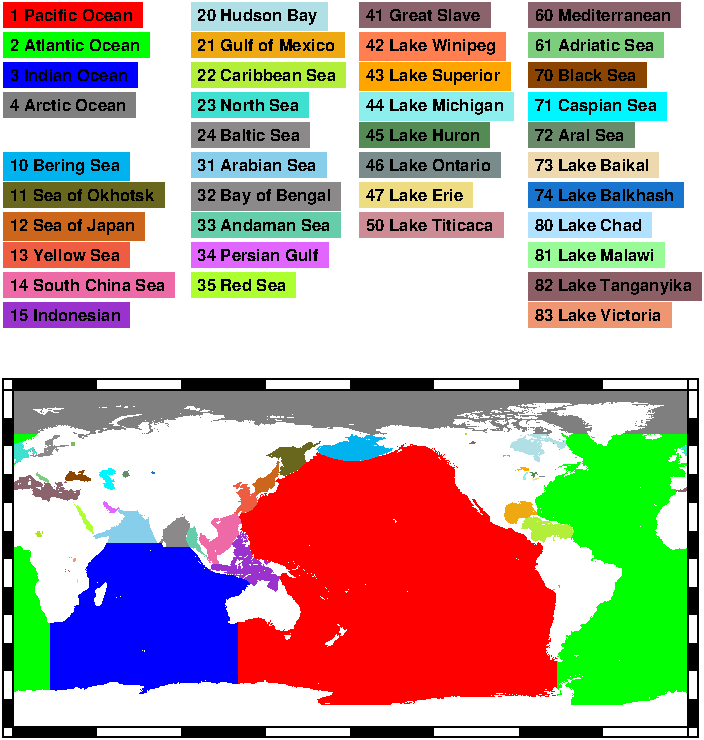
\includegraphics[width=\textwidth]{basin_codes}
\caption{Basin codes. The different colours relate to the various numerical identifiers used for each ocean basin, enclosed sea or lake.}
\label{fig:basin_codes}
\end{figure}

%%%%%%%%%%%%%%%%%%%%%%%%%%%%%%%%%%%%%%%%%%%%%%%%%%%%%%%%%%%%%%%%
\bibliography{altim}
\printindex
\end{document}

